\documentclass[glossy]{beamer}
\useoutertheme{wuerzburg}
\useinnertheme[realshadow,corners=2pt,padding=2pt]{chamfered}
\usecolortheme{shark}

\usepackage{polski}
\usepackage[utf8]{inputenc}
\usepackage{graphicx}
\usepackage{hyperref}
\usepackage{pifont}
\usepackage{ mathrsfs }
\usepackage{ amssymb }

\usepackage{tikz}
\newcommand<>{\hover}[1]{\uncover#2{%
 \begin{tikzpicture}[remember picture,overlay]%
 \draw[fill,opacity=0.4] (current page.south west)
 rectangle (current page.north east);
 \node at (current page.center) {#1};
 \end{tikzpicture}}
}

\title{Maszyny wektorów nośnych. Teoria i zastosowania.\\
		część 2: Zastosowania}
\author{mgr Agnieszka Pocha, mgr Maciej Brzeski}
\institute{Wydział Matematyki i Informatyki UJ, \\
			Katedra Metod Uczenia Maszynowego}
\date{Kraków, \today}

\begin{document}

\begin{frame}
\maketitle
\end{frame}

\begin{frame}
	\frametitle{Przypomnienie}
    \begin{center}
		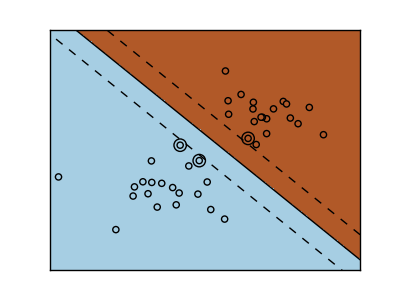
\includegraphics[scale=0.7]{plot_svm_margin_0011} \\
    	\ding{90} $w^Tx + b = 0$ \\
        $sgn(w^Tx_{new}+b)= \begin{cases} \displaystyle +1 \\ \displaystyle -1  \end{cases}$
	\end{center}    
\end{frame}

\begin{frame}
\ding{43} $w = \sum\limits_{i=1}^{m}\alpha_iy^{(i)}x^{(i)}$ 

$\alpha_i$ \ding{222} wyliczenie ze wzorku wyprowadzonego na poprzednim seminarium:

$\mathscr{L}(\alpha) = \sum\limits_{i=1}^{m}\alpha_i - \frac{1}{2}\sum\limits_{j = 1, k = 1}^{m}y^{(j)}y^{(k)}\alpha_j\alpha_k(x^{(j)})^Tx{(k)}$

będziemy szukać $\max\limits_\alpha \mathscr{L}(a)$ przy ograniczeniach:
\begin{itemize}
	\item $\alpha_i \geqslant 0$ %a_i>=0 - poprawiłem
    \item $\sum\limits_i \alpha_iy^{(i)} = 0$
\end{itemize}
Używamy w tym celu algorytmu SMO.
\end{frame}

\begin{frame}
A można prościej!

Podstawmy \ding{43} do \ding{90} i otrzymamy:
$( \sum\limits_{i=1}^{m}\alpha_iy^{(i)}x^{(i)})^Tx + b = 0$

$x$ - to tutaj nowy punkt, który chcielibyśmy sklasifikować, $x^{(i)}$ - kolejne punkty ze zbioru uczącego

zatem pytamy jaki znak miałoby poniższe wyrażenie: \\
\ding{76} $\sum\limits_i \alpha_i y^{(i)}<x^{(i)}, x>+b$

zauważmy, że w tym wzorze nie ma w ogóle $w$, zatem nie musimy go wyliczać!

$x^{(i)}$ - to są właśnie tytułowe wektory nośne
% Wektory nośne są tylko tam, gdzie a_i>0!! Generalnie musisz gdzieś wcześniej zauważyć, że tych nośnych jest niewiele (są to tylko te, które leżą na marginesach - dla losowych danych to jest niemalże stała liczba niezależna od rozmiaru danych.
% I dlatego w sumie ostatecznie można napisać, że sumujesz tylko po niezerowych a_i - w szczególności tylko dla kilku wartości wyliczas iloczyn skalarny. Ostatecznie to jedyna rzecz którą robisz - dlatego ten wzorek jest lepszy i można go łatwo zastosować dla kerneli
\end{frame}

\begin{frame}
\frametitle{Dane liniowo nieseparowalne.}
\begin{center}
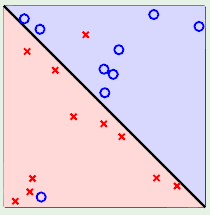
\includegraphics[]{non-separable}
\end{center}
\end{frame}

\begin{frame}
\frametitle{Overfitting.}
\begin{center}
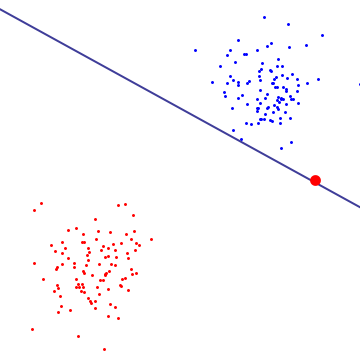
\includegraphics[scale=0.55]{overfitting}
\end{center}
\end{frame}

\begin{frame}
\frametitle{Funkcja kosztu.}

\begin{center}
$\min\limits_{w,b}\frac{1}{2}\|w\|^2+c\sum\limits_{i=1}^n\xi_i$,

pod warunkiem: $y^{(i)}[w^Tx^{(i)}+b] \geqslant 1-\xi_i $
\end{center}
% * <agnieszka.pocha@uj.edu.pl> 2016-01-16T21:53:55.102Z:
%
% co to jest to \xi_i? to to cosik sprytnego było...
% koszt przydzielenia i-temu punktowi wartości y_i. Dla punktów dobrze sklasyfikowanych jest 0, dla pozostałych - odległość od marginesu
% ^.

\begin{itemize}
\item $\xi_i$ - koszt przydzielenia i-temu punktowi wartości $y^{(i)}$. Dla dobrze sklasyfikowanych wynosi 0, dla źle sklasyfikowanych jest równa odległości od marginesu. 

\item $c$ - stała regularyzacji, przypisując jej konkretną wartość określamy, jak bardzo chcemy karać klasyfikator za błędną klasyfikację.

\item czynnik $\|w\|^2$ zapobiega overfittingowi - każe klasyfikator za zbyt duże wagi
\end{itemize}


% * <agnieszka.pocha@uj.edu.pl> 2016-01-16T21:53:42.808Z:
%
% Niestety przy tak postawionym problemie wzorek na $b$ nie działa, a nikt nie zna, takiego, co by działał. No i jakie jest rozwiązanie tego problemu?
%
% właśnie, jakie?
% na to są osobne publikacje. Mozesz zawsze zaproponowac osobne seminarium ;p na przedstawienie problemu jak sie wylicza - wydaje mi sie, ze numerycznie, tzn uczy sie go w trakcie algorytmu, podobnie jak alfy - ale głowy nie dam
% ^.

% te obrazki niewiele się różnią. Nie możesz pokazać jakiś bardziej niepraktycznych danych? ;p Jak weźmiesz jeden odstający punbkt i c->oo, to dostajesz wyjściowy problem (separuje ci możliwie idealnie), dla coraz mniejszych będzie akceptował gorsze punkty za lepszy margines (i generalizację klasyfikatora). Tutaj trochę pojawia się ten wzorek z VC - tzn dostajesz gorszy traning error, ale h jest mniejsze. 
\end{frame}

\begin{frame}
\frametitle{Parametr c. Ilustracja}
\begin{center}
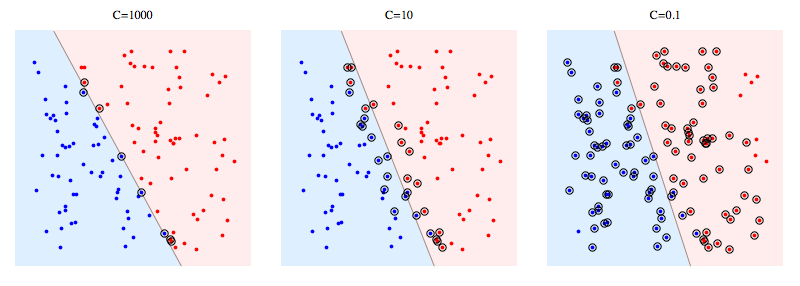
\includegraphics[scale=0.43]{c_parameter}
\end{center}
\end{frame}

\begin{frame}
\frametitle{Niezbalansowane zbiory.}
\begin{center}
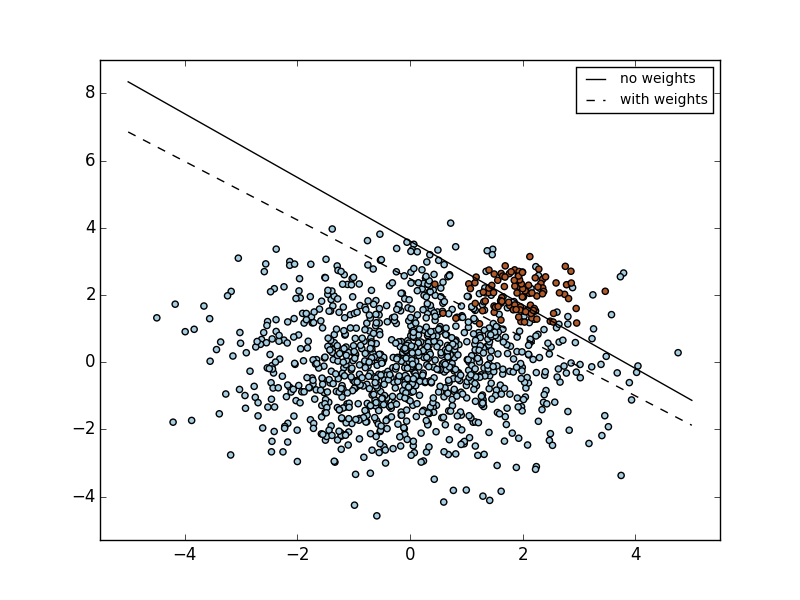
\includegraphics[scale=0.35]{unbalanced}
\end{center}
R. Batuwita, V. Palade, \textbf{Imbalanced Learning: Foundations, Algorithms, and Applications}, Haibo He and Yungian Ma (Eds.), Wiley, 2013, rozdział 6
\end{frame}

\begin{frame}
\frametitle{Wymiar Vapnika-Chervonenkisa}
Wyobraźmy sobie taką grę:
\begin{enumerate}
\item dwaj gracze ustalają liczbę punktów oraz sposób rozdzielania ich
\item gracz A ustala położenie punktów
\item gracz B nadaje im etykiety (w miarę możliwości złośliwie)
\item gracz A usiłuje rozdzielić punkty tak, by te o jednej etykiecie były po jednej stronie, a te o drugiej etykiecie po drugiej
\end{enumerate}
Wygrywa gracz A jeśli uda mu się rozdzielić punkty. Wygrywa gracz B, jeśli graczowi A się nie powiedzie.

Wymiar V-C to maksymalna liczba punktów, taka że A wygra niezależnie od poetykietowania zadanego przez B.
\end{frame}

\begin{frame}
\frametitle{Wymiar Vapnika-Chervonenkisa. Przykład sukcesu.}
\begin{center}
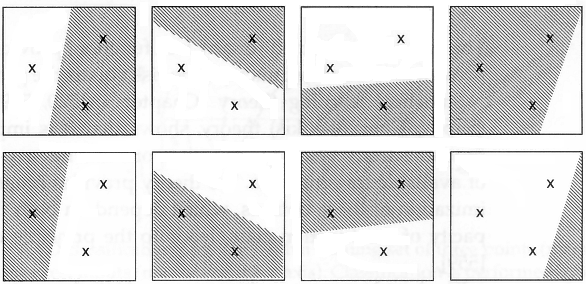
\includegraphics[scale=0.5]{success}
\end{center}
\end{frame}

\begin{frame}
\frametitle{Wymiar Vapnika-Chervonenkisa. Przykład porażki.}
\begin{center}
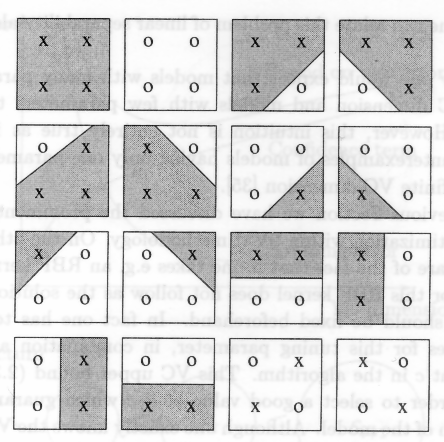
\includegraphics[]{failure}
\end{center}
\end{frame}

\begin{frame}
\frametitle{Wymiar VC. Do czego się przydaje?}
$P(test\_error \leqslant training\_error + \sqrt[]{\frac{h(\log{(\frac{2N}{h})}+1)-\log{\frac{\eta}{4}}}{N}}) = 1-\eta$

\begin{itemize}
\item $test\_error$ - błąd na zbiorze testowym
\item $training\_error$ - błąd na zbiorze trenującym
\item $h$ - wymiar VC
\item $0<\eta<1$
\item $N$ - wielkość zbioru trenującego
\end{itemize}

Ważne:
\begin{itemize}
\item $h<<N$.
\item przykłady w zbiorze trenującym i testującym są wybierane niezależnie od siebie i z tego samego rozkładu
\end{itemize}

% * <agnieszka.pocha@uj.edu.pl> 2016-01-17T16:18:33.564Z:
%
% h powinno być duże czy małe by było OK? Chyba małe, ale dlaczego. Nie widzę tego! :(
%
% h powinno być duże czy małe by było OK? Chyba małe, ale dlaczego. Nie widzę tego! :(
% h odpowiada złożoności modelu. Generalnie im większe h, tym gorsze oszacowanie (funkcja jest rosnąca ze względu na h). 
% ^.
% * <agnieszka.pocha@uj.edu.pl> 2016-01-17T16:30:50.117Z:
%
% http://www.wolframalpha.com/input/?i=plot+x*%28log%281%2Fx%29+%2B1%29+from+0+to+5
%
% ^.
\end{frame}

\begin{frame}
\frametitle{Kernel trick. Motywacja}
\begin{center}
$x$ \ding{212} $\phi(x)$ \\

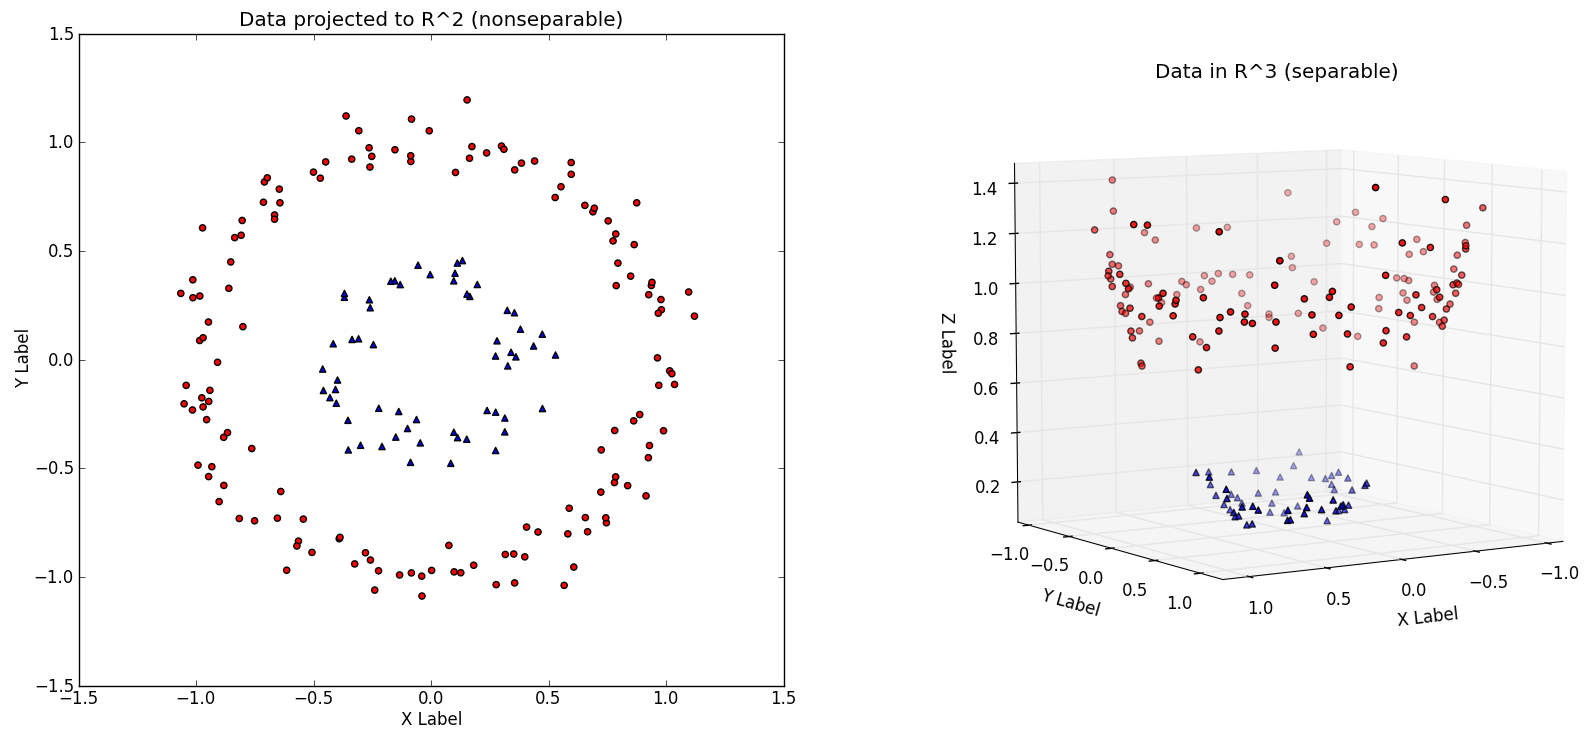
\includegraphics[scale=0.28]{kernel_space} \\
\url{http://rvlasveld.github.io/images/oc-svm/visualization.gif}
\end{center}
\end{frame}

\begin{frame}
\frametitle{Kernel trick w SVM}
Podstawmy zatem zamiast $<x^{(i)}, x>$ we wzorze \ding{76} $<\phi(x^{(i)}), \phi(x)>$ a otrzymamy:\\
\begin{center}
$\sum\limits_i \alpha_i y^{(i)}<\phi(x^{(i)}), \phi(x)>+b$
\end{center}
Wyliczenie $\phi(x)$ może być trudne/czasochłonne/niemożliwe, ale okazuje się, że policzenie $<\phi(x^{(i)}), \phi(x)>$, jest znacznie łatwiejsze/szybsze/w ogóle możliwe.
\end{frame}

\begin{frame}
\frametitle{Kernel trick. Jak to robimy?}
Wiemy, że $<\phi(x), \phi(y)>$, to jest po prostu $\phi(x)^T\phi(y)$. Definiujemy funkcję (nazywamy ją kernelem):
\begin{center}
$K(x, y):=\phi(x)^T \phi(y)$
\end{center}
\ding{76} ma teraz postać:
\begin{center}
$\sum\limits_i \alpha_i y^{(i)}K(x^{(i)}, x)+b$
\end{center}
\end{frame}

\begin{frame}
\frametitle{Kernel trick. Magia.}
Pomysł jest taki, aby w ogóle nie definiować $\phi(x)$, tylko zdefiniować od razu $K(x, y)$.
Powstaje pytanie: jak powinna wyglądać funkcja $K$?

Chcielibyśmy, by $K$ było pewną miarą "podobieństwa", tzn. jeżeli $\phi(x)$ i $\phi(y)$ leżą blisko siebie (są podobne), to $K(x, y)$ powinno być duże, natomiast jeżeli $\phi(x)$ i $\phi(y)$ leżą daleko od siebie (są niemalże ortogonalne, są niepodobne), to $K(x, y)$ powinno być bliskie $0$.

Tak jest np. gdy mamy do czynienia z kernelem gaussowskim:
\begin{center}
$K(x, y)=exp(-\frac{\|x-y\|^2}{2\sigma^2})$
\end{center}
\end{frame}

\begin{frame}
\frametitle{Kernel trick. Twierdzenie Mercera.}
Niech $X$ - zbiór jakichś punktów oraz $x^{(i)}$ to i-ty punkt w $X$. \\
Zdefiniujmy macierz $\mathscr{K}$ w taki sposób:
\begin{center}
$\forall i, j  \hspace{0.15cm} \mathscr{K}_{ij}=K(x^{(i)}, x^{(j)})$
\end{center}
Jeżeli $\mathscr{K}$ jest positive semidefinite (półdodatnio określona?) oraz symetryczna, to $K$ jest kernelem (tzn. istnieje $\phi(x)$, takie że $\forall x, y \hspace{0.15cm} \phi(x)^T\phi(y) = K(x, y)$).
\end{frame}

\begin{frame}
\frametitle{To the batmobile!}
Dlaczego SVMy są fajne?
\begin{itemize}
\item M. Fern\'{a}ndez-Delgado, E. Cernadas, S. Barro, D. Amorim; \textbf{Do We Need Hundreds of Classifiers to Solve Real World Classification Problems?}; J. Mach. Learn. Res.; January 2014;
\item szybko się uczą. naprawdę szybko.
\item "można" je douczać (online learning), są to tzw. incremental SVMs
% * <agnieszka.pocha@uj.edu.pl> 2016-01-16T23:07:51.698Z:
%
% czy można?
% nie wiem, ale strzelam że ciężko. Po zastosowaniu sztuczek znamy parametry a_i, wyliczamy tylko iloczyn skalarny (reprezentowany zwykle za pomocą kernela). Dodanie nowych przykładów chyba wymusza wyliczenie wszystkiego od 0.
% ^.
\item mają (stosunkowo) mało parametrów
\item są dosyć odporne na overfitting i nie przeraża je klątwa wielowymiarowości
\item niski wymiar Vapnika-Chervonenkisa
\item mało hyperparamaterów
\item dobrze się zachowują na rzadkich danych
\item dobrze sobie radzą, jeżeli klasy są niezbalansowane
\end{itemize}
\end{frame}

\begin{frame}
\frametitle{Jakie problemy można rozwiązywać za pomocą SVMów?}
\begin{itemize}
	\item klasyfikacja
	\item regresja: SV Regression, można poczytać w: A.J. Smola, B. Sch\"{o}lkopf, \textbf{A Tutorial on Support Vector Regression}, 1998
	\item novelty detection: one-class SVM, można poczytać w: B. Schölkopf, R. C. Williamson, A. J. Smola, J. Shawe-Taylor, J. C. Platt, \textbf{Support Vector Method for Novelty Detection}, 1999, NIPS
\end{itemize}
\end{frame}

\begin{frame}
\frametitle{Przykłady w pythonie.}
\begin{enumerate}
	\item sam proces uczenia - jak zmieniają się wektory nośne/decision boundary
  \item jakie są różnice, gdy stosujemy różne kernele
  \item multi-class classification
  \item rysowanie największego marginesu
  \item niezbalansowanie zbiory
  \item przykład dla weighted examples
  \item regression
  \item novelty detection
\end{enumerate}
\end{frame}



\begin{frame}
\frametitle{Podsumowanie}
\begin{center}
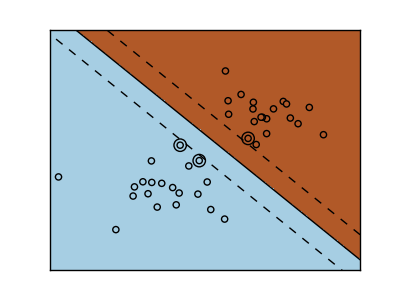
\includegraphics[scale=0.4]{plot_svm_margin_0011}
\end{center}
\begin{itemize}
\item $w^Tx + b = 0$
\item małe
\item szybkie
\item zwinne
\item dobrze radzą sobie z większością problemów
\item istnieje wiele wariacji SVMów (SVR, on-class SVM, różne kernele)
\end{itemize}
\end{frame}

\begin{frame}
\frametitle{Bibliografia}
\begin{enumerate}
\item no wikipedie, bo zawsze warto od nich zacząć
\item C. Bishop, \textbf{Pattern Recognition and Machine Learning}, 2006, Springer, rozdziały 6 (Kernels) i 7 (Kernel Models)
\item T. Hastie, R. Tibshirani, J. Friedman, \textbf{The Elements of Statistical Learning}, Springer, 2008, rozdział 12
\item Andrew Ng, CS229, Stanford, \url{http://cs229.stanford.edu/notes/cs229-notes3.pdf} \\ + jest także nagranie z wykładu
\item M. Fern\'{a}ndez-Delgado, E. Cernadas, S. Barro, D. Amorim; \textbf{Do We Need Hundreds of Classifiers to Solve Real World Classification Problems?}; J. Mach. Learn. Res.; January 2014;
\item A.J. Smola, B. Sch\"{o}lkopf, \textbf{A Tutorial on Support Vector Regression}, 1998
\end{enumerate}
\end{frame}

\begin{frame}
\begin{enumerate}
\setcounter{enumi}{6}
\item B. Schölkopf, R. C. Williamson, A. J. Smola, J. Shawe-Taylor, J. C. Platt, \textbf{Support Vector Method for Novelty Detection},
\item R. Batuwita, V. Palade, \textbf{Imbalanced Learning: Foundations, Algorithms, and Applications}, Haibo He and Yungian Ma (Eds.), Wiley, 2013, rozdział 6
\item \url{http://rvlasveld.github.io/blog/2013/07/12/introduction-to-one-class-support-vector-machines/}
\item przykłady w pythonie i pożyteczne intuicje są na scikit-learn
\item \url{http://stackoverflow.com/a/4630731}
\end{enumerate}
\end{frame}

\begin{frame}
\frametitle{Obrazki}
1. \url{http://scikit-learn.org/stable/_images/plot_svm_margin_0011.png} \\
2. \url{http://www.blaenkdenum.com/images/notes/machine-learning/kernel-methods/slightly-non-separable.png} \\
3. \url{http://yaroslavvb.com/upload/save/so-svm.png} \\
4. \url{http://yaroslavvb.com/upload/save/so-libsvm.png} \\
5. \url{http://scikit-learn.org/stable/_images/plot_separating_hyperplane_unbalanced_001.png} \\
6. \url{http://www.svms.org/vc-dimension/ScholkopfSmola2002_1-4.png} \\
7. \url{http://www.svms.org/vc-dimension/Suykens-etal2002_2-9.png}
8. \url{http://www.eric-kim.net/eric-kim-net/posts/1/imgs/data_2d_to_3d.png}
\end{frame}

\begin{frame}
\begin{center}
Dziękuję za uwagę.

Slajdy i kody można znaleźć pod \url{github/Lamiane/slajdy/semMatSts}
\end{center}
\end{frame}



\end{document}